\documentclass[letterpaper, 10 pt, conference]{ieeeconf}
\usepackage[utf8]{inputenc}
\usepackage[spanish]{babel}
\usepackage{hyperref}
\usepackage{graphicx}
\IEEEoverridecommandlockouts
\overrideIEEEmargins

\def\equationautorefname~#1\null{(#1)\null}

\title{\bf
Churn Prediction with Logistic Regression \large  \\
Intelligent Systems Technologies
}


\author{Alberto Castañeda Arana %
}


\begin{document}



\maketitle
\thispagestyle{empty}
\pagestyle{empty}


%%%%%%%%%%%%%%%%%%%%%%%%%%%%%%%%%%%%%%%%%%%%%%%%%%%%%%%%%%%%%%%%%%%%%%%%%%%%%%%%
\begin{abstract}
Churn prediction is a useful tool for businesses that need to identify customers which have a high chance of cancelling their services.
With the ability to create these predictions on demand, businesses can reduce costs of adquiring new clients by retaining the existing ones. In this project, a Logistic Regression model made from scratch was analyzed and developed to
predict if a customer will cancel a service or 'churn' given their recorded atributes. 
\end{abstract}

\section{ Introduction }
Churn refers to a regular, quantifiable process or rate of change that occurs in a business over a period of time as existing customers are
lost and new customers are added [1]. While every customer could have a different reason for unsubscribing from a service, some even personal reasons,
there are predictors that can be used in order to find out improvement areas of their operations 
so that their churn rate can become lower. \\

Given the previously mentioned existing predictors of customers, the purpose of this project is to create a tool that predicts whether a customer is likely to cancel the service
or 'churn' so that further efforts can be made to retain that customer. \\


The problem can be described as a binary classification problem where the desired output that needs to be predicted is if a given customer is likely to churn or not.
To tackle this problem, there is multiple classifcation machine learning algorithms that are able to classify binary outcomes in order to make these predictions.
For this project, a Logistic Regression model made from scratch is proposed fo its simplicity and speed. \\

Additionally, the model will be trained alongside other implementations from the SciKit framework to compare their accuracy and training speed between each other.

\section{ Theory }
\subsection{Logistic Regression}
Logistic Regression is a statistical method used to obtain the probability of a certain class existing based
on input variables that are defined for the model. \\

In Machine Learning, Logistic Regression can be used as a tool to create accurate predictions of outcomes given some predictor variable data. \\

While there are multiple types of Logistic Regression depending on what needs to be achieved, for this case a Binary Logistic Regression is used in order
to predict a churn or not churn prediction. Like the name of the model implies, the outcome will be represented by a binary value; the value being either 1, or 0.
As previously mentioned, Logistic Regression outputs a continous number between 0 and 1, which is why we must define a threshold (defined as 0.5 by default) in order to 
transform this continous value to a 0 or 1 value.
\\


\begin{figure}[thpb]
    \centering
    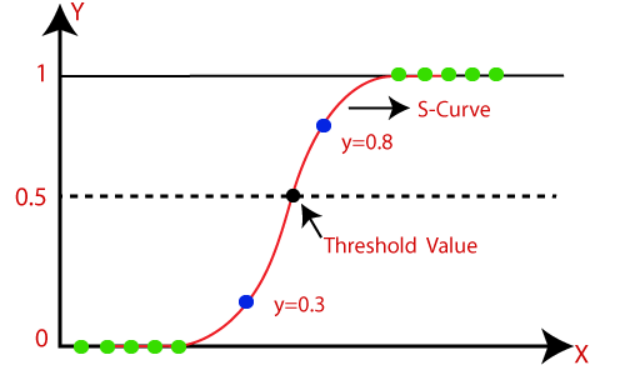
\includegraphics[scale=0.3]{figures/threshold.png}
    \caption{Logistic Regression graph with threshold for classification.}
    \label{logisticThreshold}
 \end{figure}

Using Figure 1 as an example of the previous idea, every value above 0.5 would be classified as 1 while the opposite would be classified as 0. \\

The function of Figure 1 could be represented by a sigmoid function, which has the formula:

\begin{figure}[thpb]
    \centering
    \begin{equation}
        y = g(x) = \frac {1}{1 + e^{-x}}
    \end{equation}
    \caption{Sigmoid Function}
    \label{sigmoid_formula}
 \end{figure}

 Transforming Figure 2 with the base hypothesis formula from Linear Regressions, the formula for the Logistic Regression is defined as:

 \begin{figure}[thpb]
    \centering
    \begin{equation}
        h_\theta (x) = g(\theta^Tx) = \frac{1}{1 + e^{-\theta^Tx} }
    \end{equation}
    \caption{Logistic Regression Function}
    \label{logistic_formula}
 \end{figure}

\subsection{Cost Function}
Cost functions are used to determine the minimization needed to make models have a better performance. The function reflects how much
the predicted output differs from the original output with the goal of optimizing the model. In other words, we use the cost function to measure how
close the model's predictions are to the real outputs. For binary classifcation models, a Cross-Entropy loss function is required. The formula
for such function goes as follows:

\begin{figure}[thpb]
    \centering
    \begin{equation}
        J(\theta) = - \frac{1}{m}\sum_{i = 1}^{m} y^i \log h_\theta(x^i) + (1-y^i)\log(1 - h_\theta(x^i))
    \end{equation}
    \caption{Cross-Entropy loss formula}
    \label{cost_formula}
 \end{figure}

\subsection{Gradient Descent}
Gradient Descent is an iterative optimization algorithm which finds the minimum of a diferentiable function. In this case, Gradient Descent
can be applied to the cost function of Logistic Regression to find the optimial parameters for our hypothesis. By applying the previously established
hypothesis function to the gradient descent formula, we would get:


\begin{figure}[thpb]
    \centering
    \begin{equation}
        \theta_j = \theta_j - \alpha\frac{1}{m}\sum_{i = 1}^{m}((h_\theta(x^i) - y^i)x^i_j)
    \end{equation}
    \caption{Gradient descent with Logistic Regression}
    \label{gd_formula}
 \end{figure}

\section{ Data }
\subsection{ Dataset }
For this project, the dataset chosen to train the models is a Telephone Company customer dataset provided from IBM and retrieved from Kaggle [2].
The dataset contains the Telephone Company (Telco) customer's characteristics and contract information while also indicating whether the customer departed from the company within the last month.

\subsection{ Data Analysis}

From the dataset, the proportion of how many customers were classified as churn and not churn is as follows:

\begin{figure}[thpb]
    \centering
    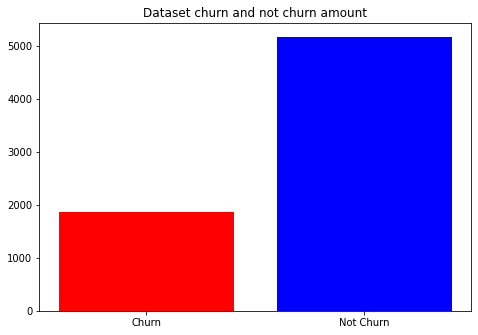
\includegraphics[scale=0.3]{figures/churn_propotion.png}
    \caption{Churn / Not Churn proportion.}
    \label{churnProportion}
 \end{figure}

As we can see on the previous figure, we have an approximate 1:3 ratio of churn and not churn customers which makes the training
contemplate both of these scenarios with sufficient data.

By doing exploratory data analysis on the dataset, the following observations were made.
\begin{itemize}
    \item CustomerID is a primary key and does not give any useful information.
    \item Gender does not seem to be a good predictor.
    \item Customer doing paper-less billing or not does not seem to be a good predictor.
    \item Senior Citizens are more likely to churn.
    \item Customers with no partners or dependents are more likely to churn.
    \item Short-term customers, or customers with lower tenure, are more likely to churn.
    \item Customers that do not have services (online security, online backup, device protection, tech support) are more likely to churn.
    \item Customers with lower total charges are more likely to churn.
\end{itemize}
By doing the previous observations, we can conclude that most of the features in the dataset can be used as a predictor with the exception of:
\begin{itemize}
    \item CustomerID
    \item Gender
    \item Paper-less billing
\end{itemize}

As such, these columns will be dropped from the feature extraction for the models fiting. \\

Additionally, empty cells in the TotalCharge column were found in some rows. For this, an approximation calculation of tenure * MonthlyCharge was done
to approximately represent the TotalCharge and to fill these empty cells.

\section{ Preprocessing}
After analyizing the data and making the previous observations, it is now time to clean and transorm the data 
in order to train our proposed models. \\

As mentioned in the previous section, we first drop columns that do not seem to give good predictors. Afterwards, since machine learning 
algorithms require purely numerical values for fitting, we must transform each categorical feature to a numerical type. To do this, we first
transform each Yes/No classification column as a binary representation (0 for no, 1 for yes) which also includes our target variable Churn.  \\

One problem is presented with some categorical values which have more than 2 possible labels. For example: the InternetService feature can possibly
have three labels (DLS, Fiber Optic, No Internet Service). To tackle this problem, one-hot encoding was used to transform these features into multiple 
numerical features. \\

\begin{figure}[thpb]
    \centering
    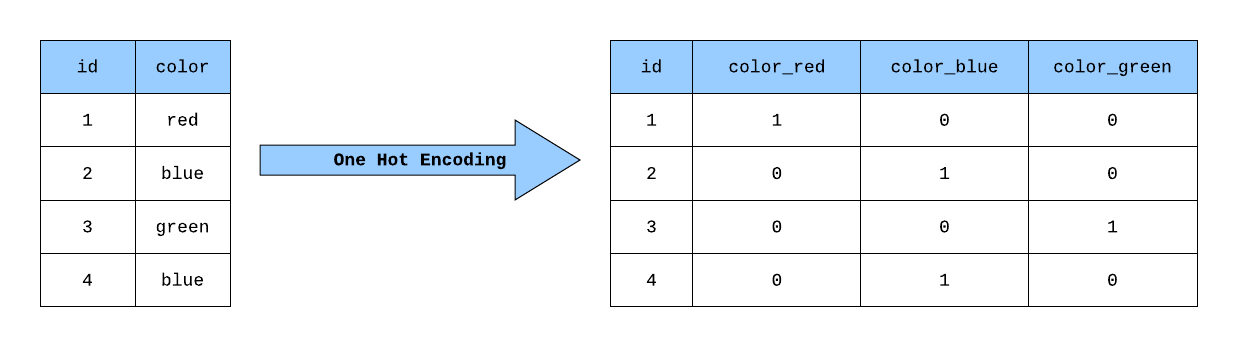
\includegraphics[scale=0.2]{figures/one_hot.png}
    \caption{One Hot Encoding transformation}
    \label{one_hot}
 \end{figure}

Additionally, as mentioned in the previous section there are some empty cells that need to be replaced. From the dataset analyisis, only the total charge feature has
these empty cells so a MonthlyCharge * tenure calculation is used to fill these cells.


Lastly, since our model will be working with a sigmoid function, we must normalize our values to prevent overflow errors that can be thrown with the exponential tending toward small numerical values on infinity.
Initially, the models did not scale the features which caused multiple overflow warnings and lower accuracy overall. \\

To do this, the StandardScaler class from the SciKit library is used to scale the training and test data.

\section{ Results }

\subsection{ Fitting }
In order to test our models, the dataset was split with 20\% of the data used for testing and 80\% for training. \\

The Logistic Regression model made from scratch was trained with 8000 epochs and a learning rate of 0.001. The following chart represents the
Cross-Entropy loss function compared to each epoch.

\begin{figure}[thpb]
    \centering
    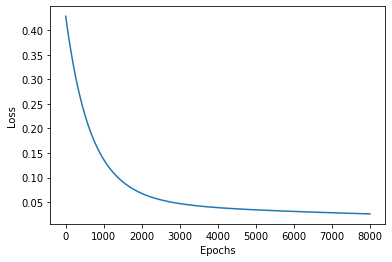
\includegraphics[scale=0.6]{figures/epochs.png}
    \caption{Epochs vs Cost Function}
    \label{epochs}
 \end{figure}


While the model can be trained with more epochs, the training time would become too big for the scope of this project. \\

\subsection{Accuracy}
After fitting each model, the following prediction accuracy percentages were given per model:
\begin{figure}[thpb]
    \centering
    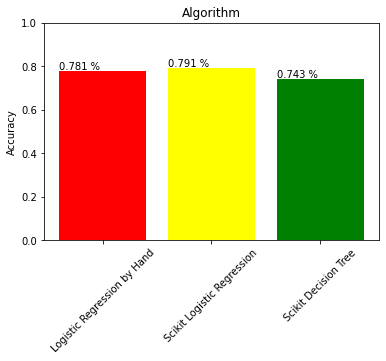
\includegraphics[scale=0.5]{figures/accuracy.png}
    \caption{Accuracy per model}
    \label{accuracy}
 \end{figure}

As seen on the plot, our Logistic Regression model got approximately 78.1 \% accuracy during testing, slightly lower than the SciKit framework
implementation. However, the previous two models consistently got ~6 \% higher accuracy than the SciKit framework implementation of a Decision Tree Classsifer. \\

\subsection{Training time}
\begin{figure}[thpb]
    \centering
    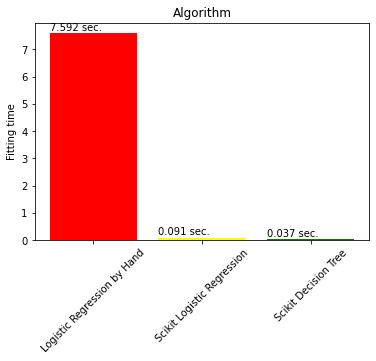
\includegraphics[scale=0.5]{figures/training_time.png}
    \caption{Training time per model}
    \label{training_time}
 \end{figure}

 As seen on the plot, our Logistic Regression model was approximately 10x time slower than other models from the SciKit framework with the same data.
 The reason for this drastic difference could be attributed to the lack of parralelization in the model made from scratch, which SciKit
 uses to improve training speed performance.

\subsection{Confusion Matrix}
\begin{figure}[thpb]
    \centering
    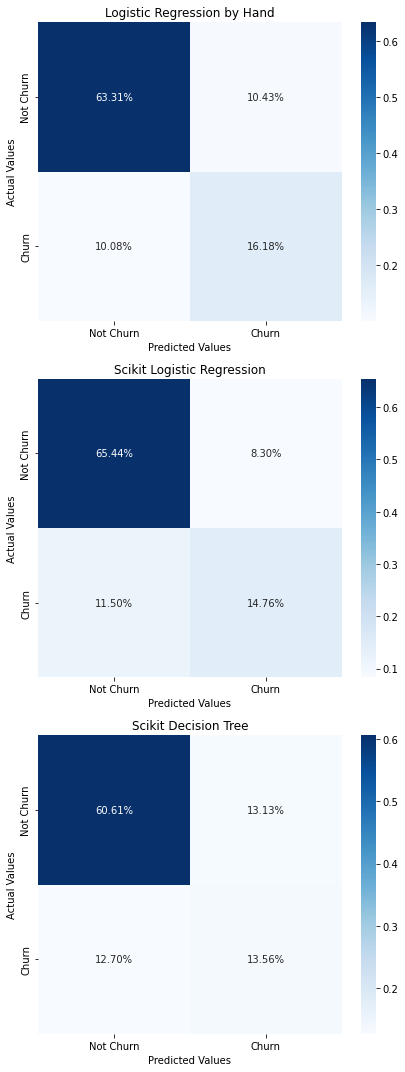
\includegraphics[scale=0.5]{figures/confusion.png}
    \caption{Confusion matrix per model}
    \label{confusion}
 \end{figure}


As seen on the previous vector of confusion matrix, the scratch Logistic Regression model has approximately equal False Negatives compared to False Positives.
On the other hand, the SciKit implementation has a higher ratio of False Negatives compared to False Positives.
Lastly, the SciKit implementation of Decision Tree ratio of False Negatives to False Positives is similar to the first model but higher. 

\subsection{Receiver Operating Characteristic Curve}

A Receiver Operating Curve (ROC) is a graph showing the performance of a classifcation model at all classifcation thresholds. This curve
plots two parameters: True Positive Rate and False Positive Rate. \\

The curve is compared with the threshold and a larger the area under the curve (AUC) is usually better.

\begin{figure}[thpb]
    \centering
    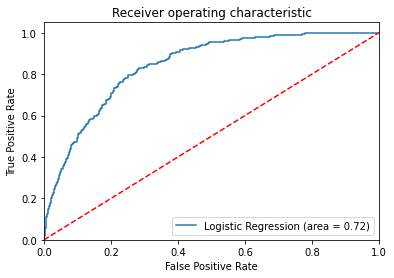
\includegraphics[scale=0.5]{figures/LOR.png}
    \caption{Scratch Logistic Regression model ROC}
    \label{LOR}
 \end{figure}

 
\section{ Discussion }
While the theory was applied succesfully and the scratch Logistic Regression model got pretty similar results to that of the SciKit implementation,
all of the models could have better accuracy (with an average of 80 \% at best). A standalone query script was developed additionally to 
obtain input data from the user to create a predition with the scratch Logistic Regression model. Some tests were done with this query program
to intentionally trigger Churn and Not Churn predictions. However, most of these queries resulted in False Negatives. The previous experiments 
imply that the models may be overfitting with the dataset. Other approaches in the state of the art which use the same dataset were investigated and it was found
that these approaches resulted in approximately similar accuracy percentages. This implies that the problem could be from the dataset itself. 
Improvements could be made to the models by providing more data especially combining from different sources.

%%%%%%%%%%%%%%%%%%%%%%%%%%%%%%%%%%%%%%%%%%%%%%%%%%%%%%%%%%%%%%%%%%%%%%%%%%%%%%%%
\begin{thebibliography}{99}
\bibitem{} churn. 2011. In Merriam-Webster.com. Retrieved March 22, 2022, from https://www.merriam-webster.com/dictionary/hacker
\bibitem{} Telco Customer Churn, 2018. In Kaggle.com. Retrieved March 22, 2022, from https://www.kaggle.com/blastchar/telco-customer-churn
\end{thebibliography}

%%%%%%%%%%%%%%%%%%%%%%%%%%%%%%%%%%%%%%%%%%%%%%%%%%%%%%%%%%%%%%%%%%%%%%%%%%%%%%%%

\end{document}
